\subsection{Building blocks: the Enclosed Tesselation}
\label{ssec:ss_et}

% What
This section proposes a novel and theoretically-informed delineation of space to
support the development of spatial signatures.
% Why % Spatial unit is a big deal
Since spatial signatures are conceptualised as highly granular in space,
considering the ideal unit of analysis at which to measure them is of utmost
importance.
%
This step is worth spending enery and effort for two main reasons.
%% If improper --> MAUP big time
First, if ignored, there is an important risk of incurring the modifiable areal
unit problem (MAUP, \citealp{openshaw1981modifiable}). The urban fabric is not a
spatially smooth phenomenon; rather, it is lumpy, irregular and operates at very
small scales.
%
Choosing a spatial unit that does not closely match its distribution will
subsume interesting variation and will hide features that are at the very heart
of what we are trying to capture with spatial signatures.
%% If done right --> a direct way to learn about geography
Second, and conversely, we see adopting a meaningful unit a step of analysis
itself. Rather than selecting an imperfect but existing unit to try to
characterise spatial signatures, delineating our own is an opportunity in itself
to learn about the nature of urban tissue and better understand issues about
distribution and composition within urban areas.

% How: Requirements of a good unit
Let us first focus on what is required from an ideal unit of analysis for
spatial signatures. We need a partition of space into sections of built
\textit{and} lived environment that can later be pieced together based on their
characteristics. The result will feed into an organic delineation that captures
variation in the appearance and character of urban fabric as it unfolds over
space.
%
To be more specific, a successful candidate for this task will need to fulfill
at least three features: indivisibility, internal consistency, and exhaustivity.
%% Undivisable: like the atom for urban fabric
An ideal unit will need to be \textit{indivisable} in the sense that if it were
to be broken into smaller components, none of them would be enough to capture
the notion of spatial signature.
%% Internally consistent: contain only one type of fabric
Similarly, every unit needs to be \textit{internally consistent}: one and only
one type of signature should be represented in each observation.
%% Exhaustive: every portion of a geography should be covered and assigned into
%a single unit
Finally, the resulting delineation needs to be geographically
\textit{exhaustive}. In other words, it should assign every location within the
area of interest (e.g. a region or a country) to one and only one class.

% Existing options
The existing literature does not appear to have a satisfying candidate to act as
the building block of spatial signatures.
%
Without attempting an exhaustive review, an endeavour beyond the scope of this
article, the vast majority of existing approaches to delineate meaningful units
of urban form and function fall within one of the following three categories.
%% Administrative areas (cite Taubenbock 2020)
The first group relies on \textit{administrative} units such as postcodes,
census geographies or municipal boundaries (e.g. \citealp{taubenbock2020}).
%
These are practical as they usually are readily
available. However, their partition of space is usually driven by different
needs that rarely align with the measurement of spatial signatures, or indeed
those of any morphological or functional urban process.
\cite{taubenbock2019new} even argue that
``administrative units obscure morphologic reality''.
%% Uniform grids (cite papers on imagery for squared grids and mention H3)
An emerging body of work relies on granular, \textit{uniform grids} as the main
unit of analysis (e.g. \citealp{jochem2020}). This choice is usually explicitly or implicitly motivated
by the lack of a better, bespoke partitioning; the use of input data distributed
in grids (e.g. satellite imagery); and the assumption that, with enough
resolution, grids can be organically aggregated into units that match the
processes of interest.
%% Morphometric units --> MF to fill in here
A third approach followed mostly by the literature on urban morphology relies on
the definition of morphometric units. These include street segments
\citep{araldi2019}, plots \citep{bobkova2019}, building footprints
\citep{schirmer2015}, or constructs such as the sactuary area
\citep{mehaffy2010urban,dibble2019origin}.
% Not a criticism of these approaches, they're built for something else
In all these cases, the
choice is justified by the particular application in which it takes place.
However none of these approaches meet the three characteristics we require for
spatial signatures.
%
Administrative boundaries are exhaustive but rarely indivisable or consistent
when it comes to urban form, usually grouping very different types of fabric
within a single area.
%
Uniform grids are also exhaustive but, similarly to administrative definition,
the arbitrariety of their delineation with respect to urban form usually leaves
them divisable and internatlly inconsistent.
%
Morphometric units are the most theoretically appealing since they are built to
match the distribution of urban features and are usually granular enough to
warrant internal consistency and indivisibility. Most of them are however not
exhaustive as they are anchored to particular elements of the build environment,
such as streets or building footprints, which do not provide full coverage.
Plots would theoretically meet all characteristics but can be problematic due to
their variable definition leading to different geometric representations
\citep{kropf2018plots}.

% Proposal: the ET
We propose the development of a new spatial unit that we term the
\textit{enclosed tessellation cell} (EC).
%% One liner of what it is
An EC is defined as:
\begin{theorem}
        The portion of space that results from growing a morphological
tesselation within an enclosure delineated by a series of natural or built
barriers identified from the literature on urban form, function and perception.
\end{theorem}
%% Process of delineation:
Let us unpack this concept a bit further. ECs result from the combination of
three sequential steps (Figure \ref{fig:et_diagram}).

\begin{figure}
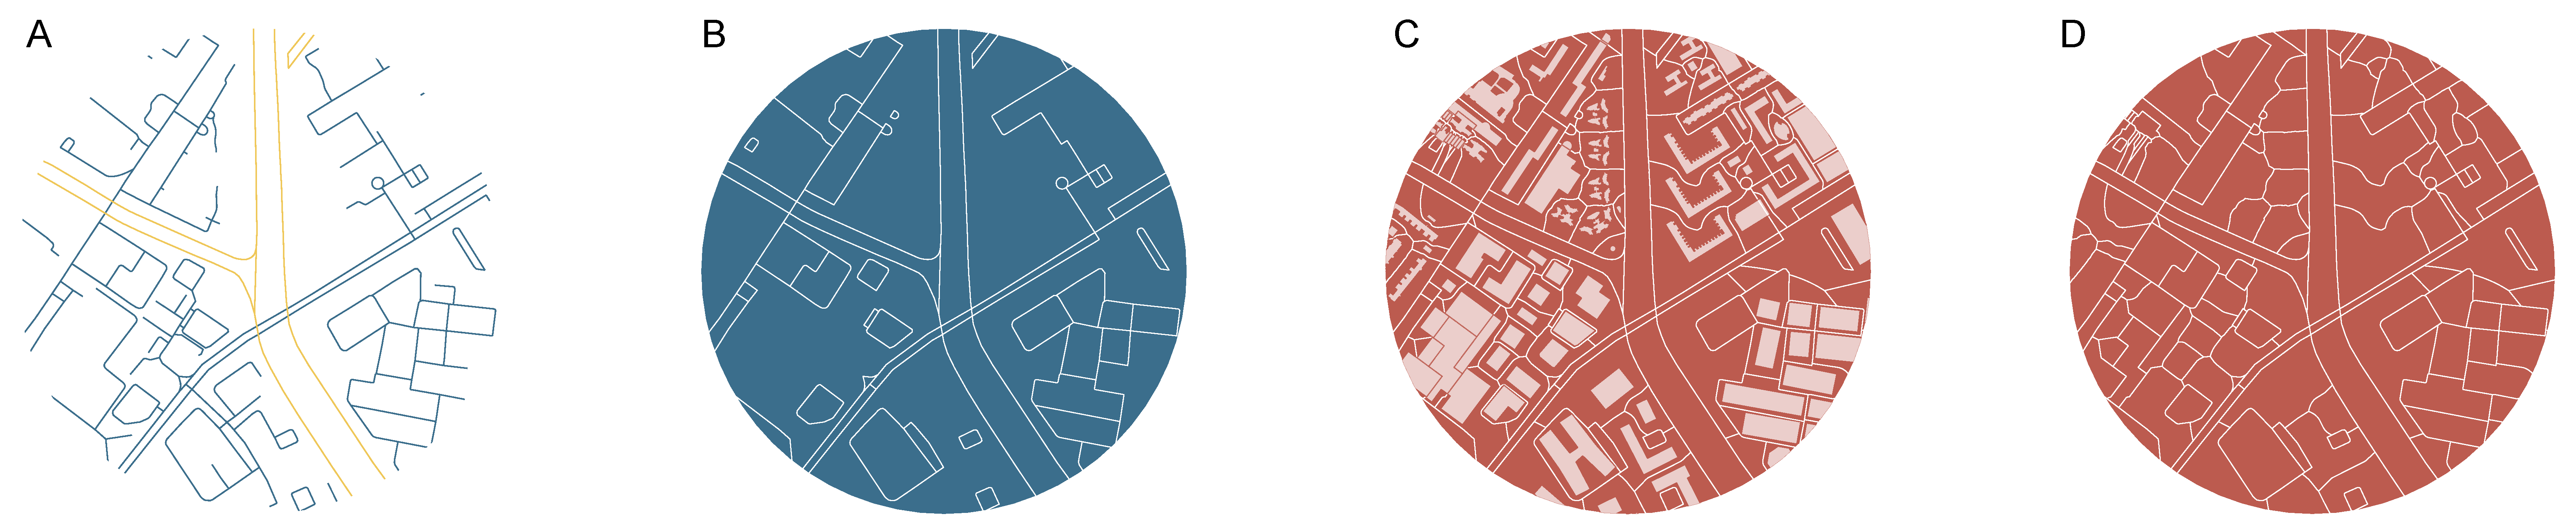
\includegraphics[width=\linewidth]{figures/et_diagram.pdf}
\caption{Diagram illustrating the sequential steps leading to the delineation of
enclosed tessellaion. From a series of enclosing components, where blue are streets and
yellow river banks (A), to enclosures (B),
incorporation of buildings as anchors (C) to final tessellation cells (D).}
\label{fig:et_diagram}
\end{figure}


%%% Gather all enclosing features (streets, rivers, railways, etc.)
First, they rely on a set of enclosing components: features of the landscape
that divide it in smaller, fully delimited portions. The list of what should be
counted as enclosing is informed by theory and, as we will see below, may vary
by context. But, as an illustration, it includes elements such as the street
network, rivers and coastlines, or railways.
%%% Build enclosing geography
Second, these enclosing features are integrated into a single set of boundaries
that partition the geography into smaller areas. In some cases, they will be
small, as with urban blocks in dense city centres; in others, they will be
larger in size, as in rural sections with lower density of enclosing features.
We call each of this fully delimited areas an enclosure.
%%% subdivision it based on building presence
Third, enclosures are further subdivided using a morphological tesselation
\citep{fleischmann2020morphological}
that exhaustively partitions space based on a set of building footprints,
which are used in this context as anchors to draw catchment polygons.
%%
This process generates geographical boundaries for a given area that result in a
new spatial unit. This unit provides full geographical coverage without any
overlap.
%
Since the essence of the approach resides in growing a tessellation inside a set
of enclosing features, we call the resulting areas ``enclosed tesselation
cells''.

%% Two foundational blocks:
The enclosed tessellation (ET) intersects two perspectives of how space can be
understood and organised.
%
%%% Enclosures (delimitters)
The first relies on the use of features that \textit{delimit} the landscape and
partition it into smaller, fully enclosed portions. These include the road and
street networks, but also others such as railways or rivers. Each feature is
conceptualised as a line that acts as a boundary, dividing space into what falls
within each of its sides.
%
A long tradition in the literature on urban perception relies on
variations of these delimiters. Prominent
early examples include the edges and paths highlighted by \cite{lynch1960} as
two of the five core elements that define legibility and imageability of a city;
as well as the later work inspired by this framework (e.g. \citealp{filomena2019a}).

%%% Building (subdelimitters) --> use morphometric lit to justify why buildings
%are so relevant
The second perspective that ET integrate is a vision organised around
\textit{anchors}. In this view, space arises in-between
a discrete set of relevant features. Unlike delimiters, these elements do not
partition space per se, but instead act as origins to which the rest can be
``attached''.
%
The choice of anchors might vary by context but, in this case, the literature on
morphometrics has extensive evidence to support the use of buildings as the
primary feature \citep{hamaina2012a, usui2013estimation, schirmer2015}.

% [Build illustration in the description]

% Why --> meets every requirement and extends the previous state-of-the-art
The combination of delimiters and anchors as the parsers of space make ECs an
ideal spatial unit to study spatial signatures, one which
meets the three requirements we outlined above.
%
They are indivisable in that a single EC will contain no delimiters, at most a
single anchor, and potentially none.
%
They are also internally consistent because they are delineated as the area
within the delimiters that contain at most one anchor.
%
And finally ECs are exhaustive in that every location within the area of
interest is assigned to one and only one EC, providing full geographical
coverage without any overlap.
